\section{Method}
\label{sec:method}

The process that allows the development of stratification can be defined by the potential energy anomaly (PEA, $\Phi$). This parameter is a quantitative measure of stratification and represents the work required per unit volume to completely mix
the water column $[Jm^{-3}]$. \\

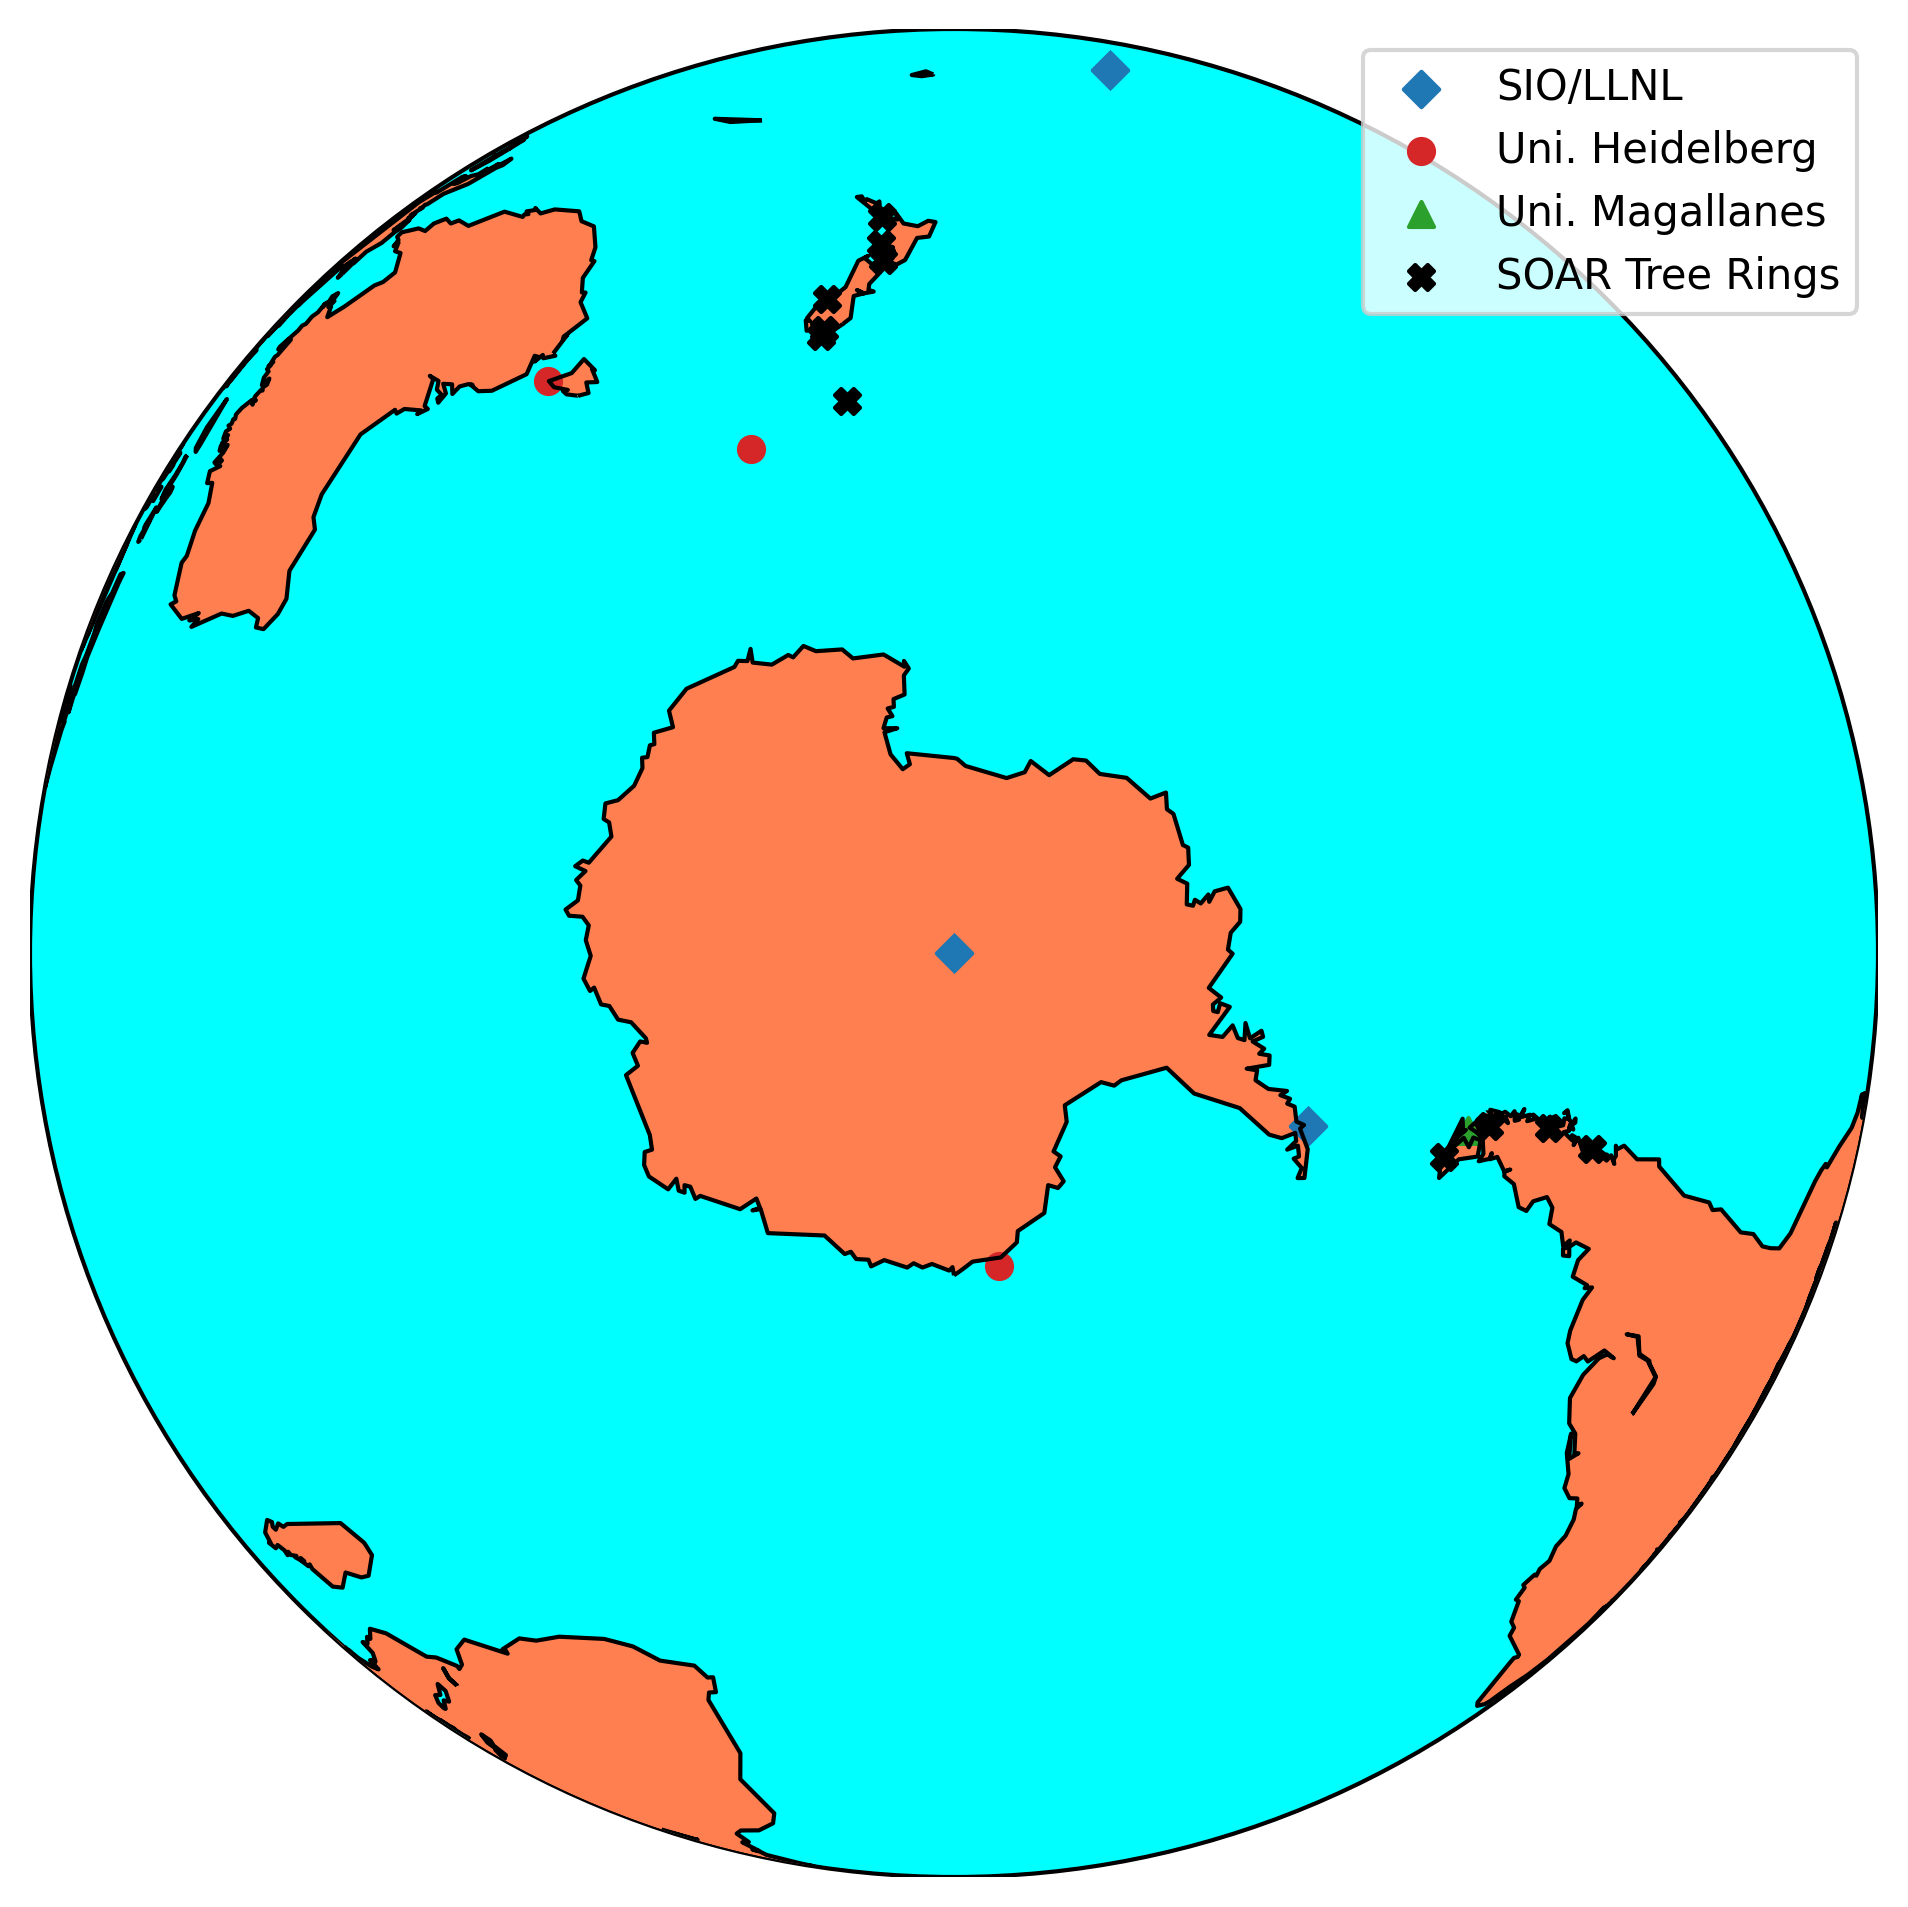
\includegraphics[width=0.5\textwidth]{/mnt/c/Users/clewis/IdeaProjects/GNS/01_science_projects/01_interlab_comparison/03_outputs/plots/newmap.png}

\noindent where z is the water column depth (m), h is the mixed layer thickness (m), g=9.81 (m $\rm s^{-2}$) is the gravitational acceleration, $\bar{\rho}$ is the water column mean density determined from temperature and salinity profiles, $\rho(z)$ is the density profile determined from temperature and salinity 
profiles. 